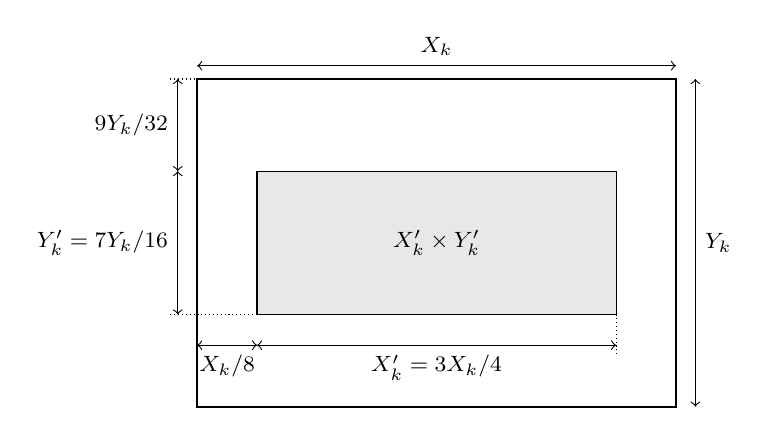
\begin{tikzpicture}[x=0.19cm,y=-0.13cm,font=\footnotesize]
  % subband of 32 x 32 units; window x0 = X/8 = 4, width 3X/4 = 24; y0 = 9Y/32 = 9, height 7Y/16 = 14
  \draw[line width=0.7pt] (0,0) rectangle (32,32);
  \fill[gray!18] (4,9) rectangle (28,23);
  \draw (4,9) rectangle (28,23);
  \node at (16,16) {$X'_k \times Y'_k$};
  \draw[<->] (0,-1.3) -- node[above] {$X_k$} (32,-1.3);
  \draw[<->] (33.3,0) -- node[right] {$Y_k$} (33.3,32);
  \draw[<->] (0,26) -- node[below] {$\floor{X_k/8}$} (4,26);
  \draw[<->] (4,26) -- node[below] {$X'_k = \floor{3X_k/4}$} (28,26);
  \draw[<->] (-1.3,0) -- node[left] {$\floor{9Y_k/32}$} (-1.3,9);
  \draw[<->] (-1.3,9) -- node[left] {$Y'_k = \floor{7Y_k/16}$} (-1.3,23);
  \draw[densely dotted] (0,26) -- (0,32) (28,23) -- (28,27);
  \draw[densely dotted] (-1.8,0) -- (0,0) (-1.8,23) -- (4,23);
\end{tikzpicture}
